\documentclass[conference]{IEEEtran}
\IEEEoverridecommandlockouts
\usepackage{cite}
\usepackage{amsmath,amssymb}
\usepackage{graphicx}
\usepackage{booktabs}
\usepackage{multirow}
\usepackage{xcolor}
\usepackage{url}
\usepackage[hidelinks]{hyperref}
\graphicspath{{../figures/}}
\newcommand{\sys}[1]{\textsc{#1}}

\begin{document}

\title{CleanTech Research Crew: A Multi-Agent Retrieval-Augmented System over the Model Context Protocol}

\author{\IEEEauthorblockN{Asad Khan}
\IEEEauthorblockA{CSC 583 Natural Language Processing, Fall 2026 \\
DePaul University, Chicago, IL \\
Final Project (Default)}}

\maketitle

\begin{abstract}
We build and rigorously evaluate an agentic question-answering system over the Cleantech Media Dataset
(20{,}111 articles). A Part~1 baseline, a LangGraph ReAct agent with a Chroma retriever and a summarizer, is
extended with six components: a from-scratch BM25 fused with dense retrieval by Reciprocal Rank Fusion and
cross-encoder reranking; tools served over the Model Context Protocol with a hand-written client; a
planner/parallel-researcher/writer/critic crew with conversation memory; input and output guardrails; ASD-STE100
answers with a rule-based compliance checker; and OpenAlex scholarly search. On 50 multi-document questions,
scored with retrieval metrics and a cross-family LLM judge (GPT-5.5, test-retest $\kappa=0.82$), retrieval
raises key-fact recall from 0.47 to 0.67, and BM25 beats dense embeddings (MRR 0.64 vs 0.54). The crew finds
17\% more of the referenced articles, yet a single ReAct agent writes equally good answers at one eighth of the
cost. STE answers triple readability but lose about 8\% of the reference facts, and the critic loop has no
significant effect. Ablations, an error-analysis-driven second version and bootstrap confidence intervals
make each of these trade-offs measurable.
\end{abstract}

\begin{IEEEkeywords}
retrieval-augmented generation, agentic AI, multi-agent systems, Model Context Protocol, BM25, LLM-as-a-judge, ASD-STE100
\end{IEEEkeywords}

\section{Introduction}
Retrieval-augmented generation (RAG) grounds a language model's answer in documents retrieved at query time
\cite{lewis2020rag}. Agentic RAG goes one step further: the model decides \emph{when} and \emph{what} to
retrieve, calling tools in a reason--act loop \cite{yao2023react}. This project builds such a system for the
Cleantech Media Dataset \cite{lipenkova2024cleantech}, 20{,}111 news articles on renewable energy,
storage, mobility and climate policy, and asks a practical question: \emph{which parts of a modern agentic
stack actually improve answers to hard, multi-document questions, and which only add cost?}

The work follows the three parts of the assignment. Part~1 builds a baseline agent with the required
retriever and summarizer tools in LangGraph \cite{langgraph}. Part~2 adds six extensions, written from
scratch where possible: (E1) hybrid retrieval with a hand-written BM25 \cite{robertson2009bm25} fused with
dense search by Reciprocal Rank Fusion \cite{cormack2009rrf} and a cross-encoder reranker; (E2) all tools
served over the Model Context Protocol (MCP) \cite{anthropic2024mcp} with a hand-written client; (E3) a
multi-agent crew of a planner, parallel researchers, a writer and a critic, with conversation memory;
(E4) input and output guardrails; (E5) answers in ASD-STE100 Simplified Technical English
\cite{asdste100}, following Karpathy's suggestion \cite{nikhil2026karpathy}, verified by a rule-based checker;
and (E6) a scholarly-search tool over OpenAlex \cite{priem2022openalex}. Part~3 (Option~A of the assignment) evaluates seven systems, including two simple baselines, on
the 50-question \emph{CleanTech-50answers} test set, scoring retrieval against the referenced articles and
answers against the desired outputs with lexical, semantic and LLM-as-judge metrics
\cite{zheng2023judge}, with bootstrap confidence intervals, paired significance tests and ablations.

\section{Data}
\subsection{Corpus and cleaning}
Each article's \texttt{content} field is a stringified Python list of paragraphs. Two scraping artefacts were
found and fixed. First, about 20\% of articles contain one ``blob'' paragraph that is the whole article
concatenated, followed by the same paragraphs again; any paragraph that contains at least two other
paragraphs verbatim is dropped, which removes 7.8\% of the characters. Second, punctuation was tokenised by
the scraper (\textit{Slovakia' s}, \textit{`` This}) and is re-joined so that BM25 sees normal words.

\subsection{Chunking}
Articles are packed paragraph by paragraph into chunks of at most 250 words (about 330 tokens, inside the
512-token limit of the encoders), with the last paragraph repeated in the next chunk when it is short. Each
chunk is embedded with its article title prepended, a \emph{contextual chunk header} that keeps short
paragraphs attributable to their project. The result is 82{,}302 chunks (median 221 words, 4.1 per article).

\subsection{Test sets}
The official RAG evaluation set has 23 rows (21 unique single-article factoid questions); 19 link to an
article in the corpus. The course's \emph{CleanTech-50answers} set has 50 multi-document synthesis questions
in eight topics, each with a desired output and 1--5 referenced article ids (2.04 on average); all 29
referenced articles are in the corpus. Notably, all of them were published within four days
(1--4 September 2023), so each question is written around a few specific articles, while the system searches
all 20{,}111.

\section{System Design}
Fig.~\ref{fig:arch} shows the final architecture.

\begin{figure*}[t]
\centering
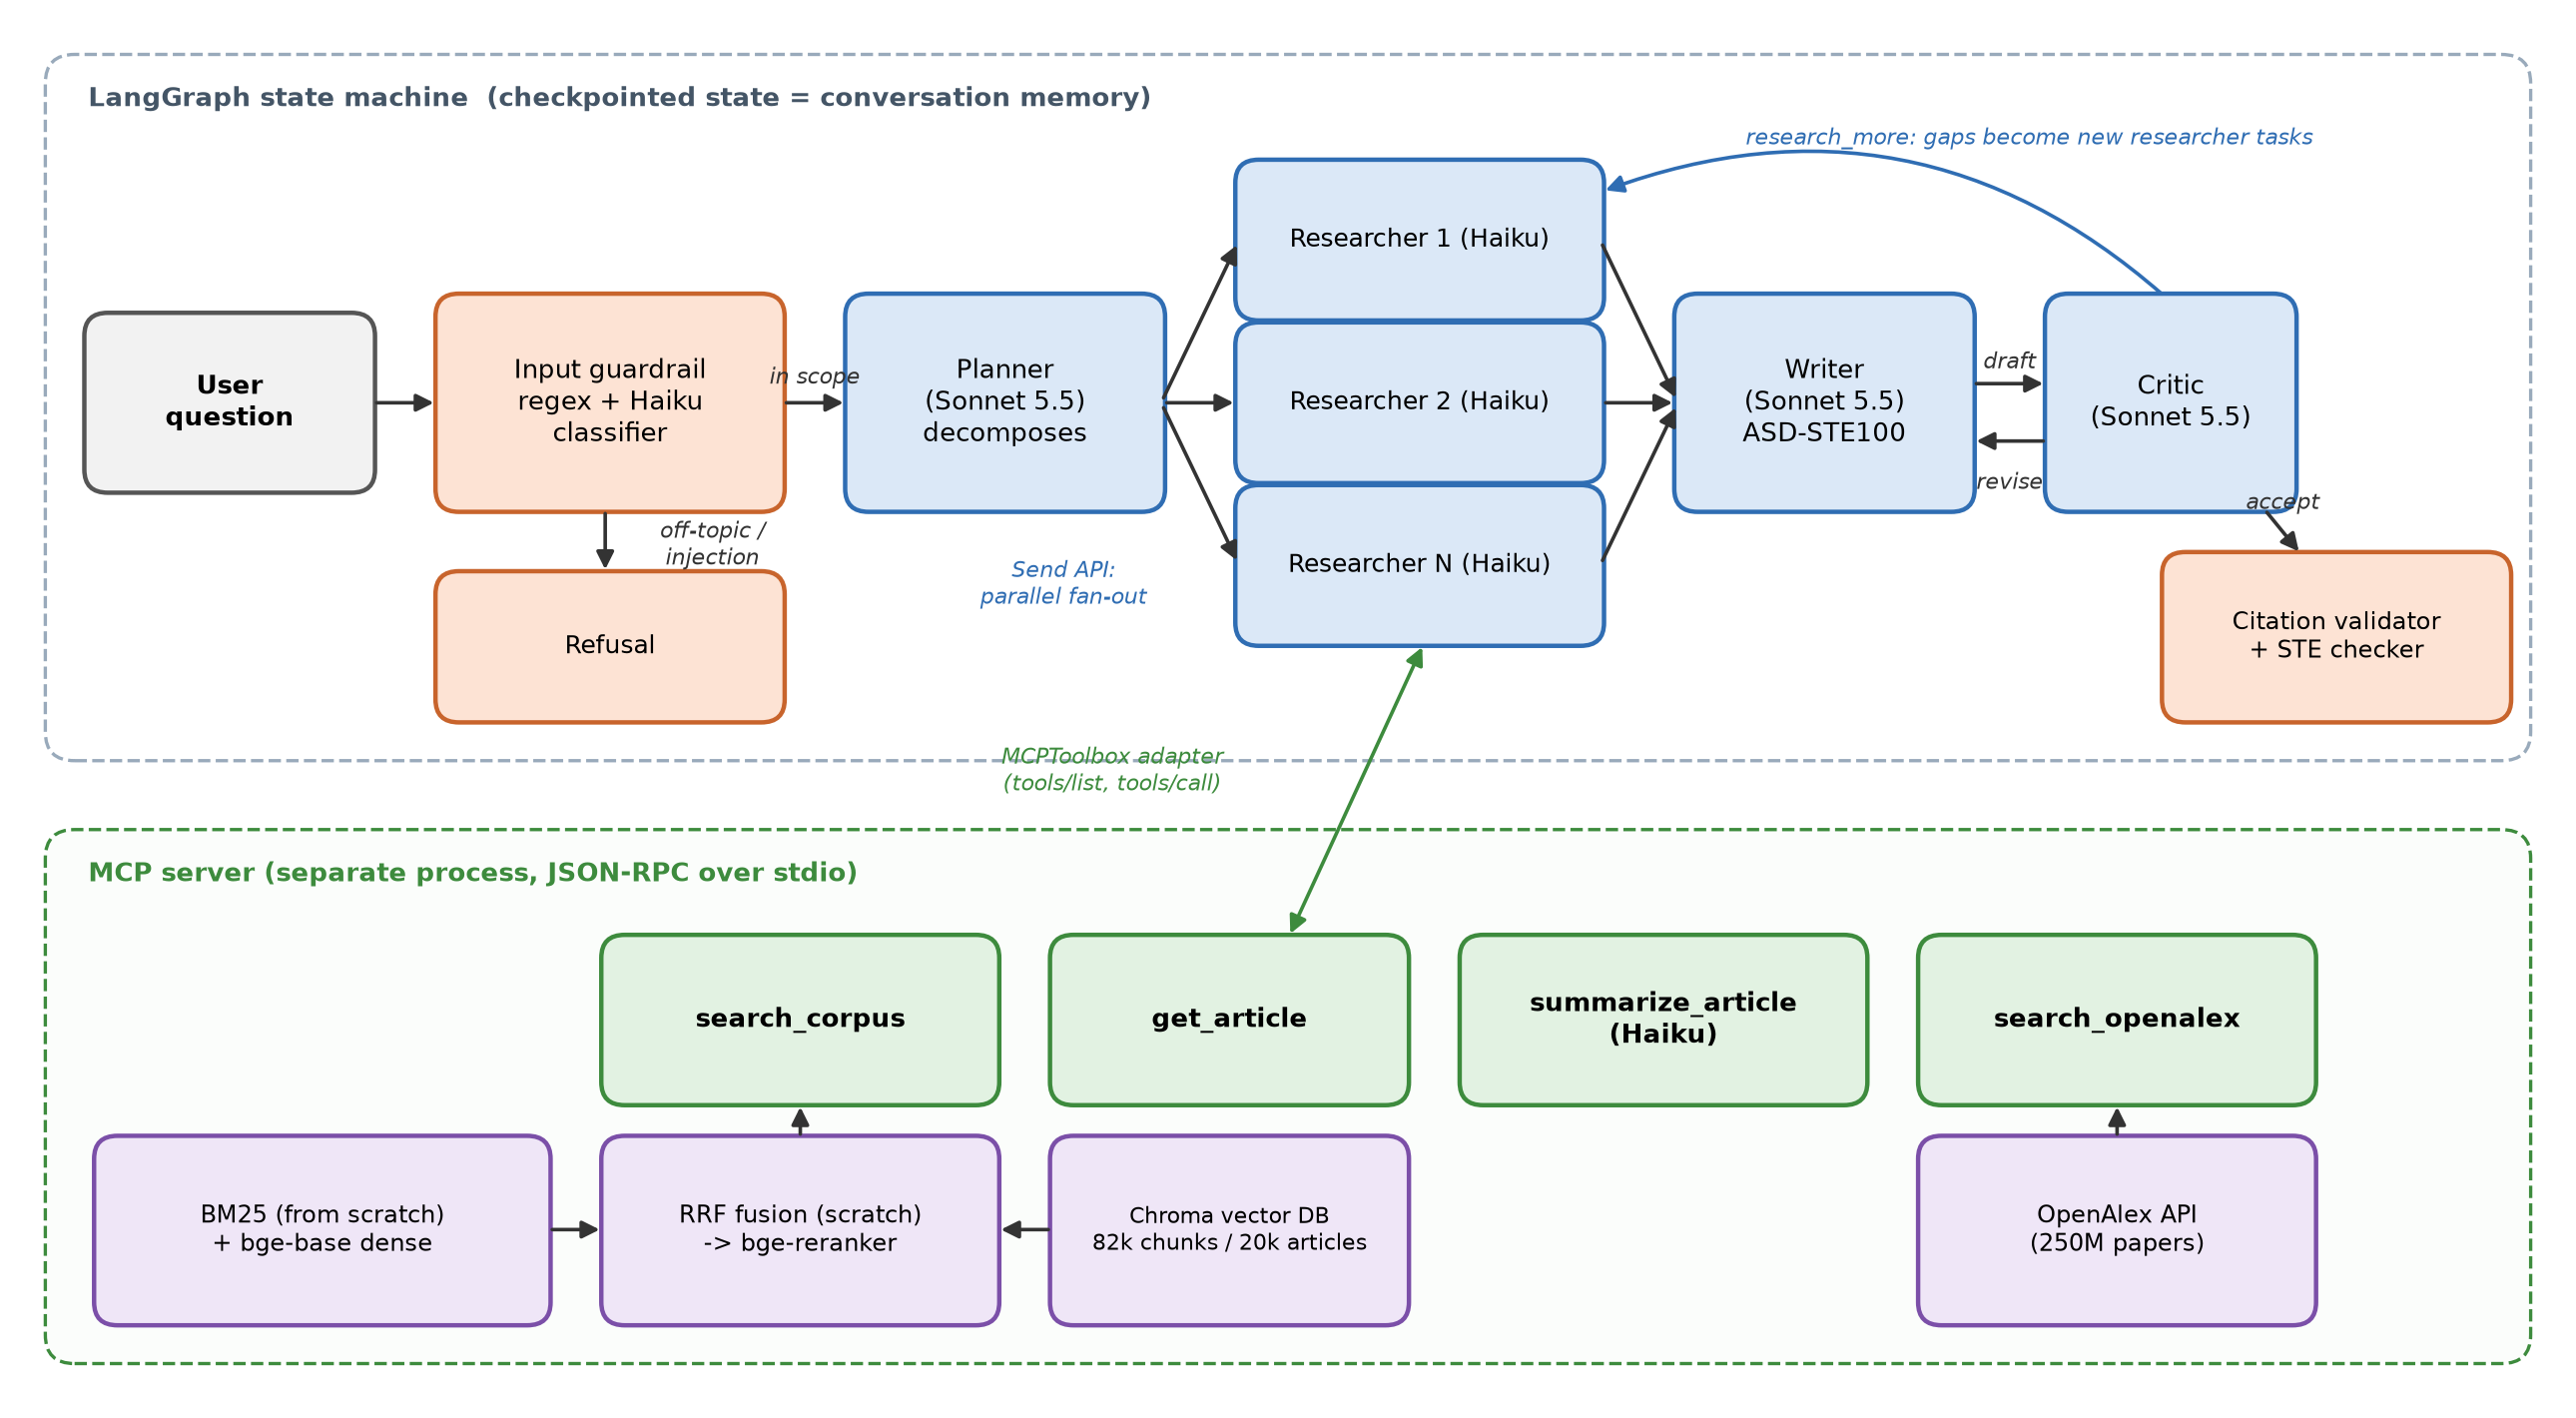
\includegraphics[width=0.86\textwidth]{architecture.png}
\caption{System architecture. The orchestration is a LangGraph state machine (top); all tools live in a
separate MCP server process (bottom). Orange: guardrails; blue: LLM agents; green: MCP tools; purple: data
and indexes.}
\label{fig:arch}
\end{figure*}

\subsection{Part 1: Baseline agent}
Chunks are embedded with \texttt{bge-base-en-v1.5} \cite{xiao2024cpack} (768-d, normalised; 45 minutes on
an Apple M4 GPU, cached) and stored in a persistent Chroma collection with an HNSW cosine index. The
baseline is LangGraph's prebuilt ReAct agent driven by Claude Sonnet~5.5 with two tools:
\texttt{retrieve(query)}, which returns the top-5 chunks labelled with article ids, and
\texttt{summarize(text, focus)}, a query-focused summary by Claude Haiku~5.5. The agent decides how often
to search, then answers in 120--250 words with an article id after each fact.

\subsection{E1: Hybrid retrieval}
BM25 is implemented from scratch on a sparse document--term matrix. Tokens are lower-cased, stop-word
filtered and Porter-stemmed, keeping numerals such as \texttt{2.3} and compounds such as
\texttt{long-duration}. With $k_1{=}1.5$ and $b{=}0.75$, the full BM25 weight of every stored
(chunk, term) pair is pre-computed, so scoring a query is a sum of a few sparse columns (4\,ms over 82k
chunks). Reciprocal Rank Fusion, also from scratch, merges the BM25 and dense top-50 lists with
$\mathrm{RRF}(d)=\sum_r 1/(60+\mathrm{rank}_r(d))$, using ranks only, so the two score scales never
need calibration. The fused top-30 is re-scored by the cross-encoder \texttt{bge-reranker-base}
\cite{nogueira2019passage}, and at most two chunks per article are kept. The larger
\texttt{bge-reranker-v2-m3} was tested first but was 9$\times$ slower (8.1\,s per query) with no recall
gain, too slow for agents that search about ten times per question.

\subsection{E2: Model Context Protocol}
All tools moved into an MCP server (official Python SDK, v2) that runs as a separate process and speaks
JSON-RPC over stdio. It exposes \texttt{search\_corpus} (E1), \texttt{get\_article},
\texttt{summarize\_article} (the Part~1 summarizer, now server-side) and \texttt{search\_openalex} (E6),
each with a JSON schema. The server loads the indexes once in a lifespan hook, serialises GPU access with a
lock (parallel researchers otherwise crashed PyTorch's non-thread-safe MPS backend), and caches LLM and
web results on disk. The client, \texttt{MCPToolbox}, is written from scratch: it spawns the server,
performs the \texttt{initialize} handshake, lists tools, and wraps each schema as a LangChain tool whose
coroutine issues \texttt{tools/call}. Results are returned twice: as compact JSON for the model and as a
structured \emph{artifact} the orchestrator uses for evidence tracking. Because the SDK's cancel scopes must
be closed by the task that opened them, and Jupyter runs each cell as a new task, the session lives in a
dedicated owner task.

\subsection{E3: Multi-agent orchestration and memory}
The crew is a LangGraph \texttt{StateGraph} with six nodes. The \textbf{planner} (Sonnet) rewrites the
question to stand alone, using the conversation history, and splits it into 1--4 entity-specific
sub-questions, each with 2--3 keyword queries; it also decides whether scholarly evidence is useful. Through
LangGraph's \texttt{Send} API, one \textbf{researcher} per sub-question runs \emph{in parallel}: a Haiku ReAct
agent that calls the MCP tools and writes cited notes. The \textbf{writer} (Sonnet) synthesizes one answer
from all notes and passages, citing an article id after every fact. The \textbf{critic} (Sonnet) checks every
claim and number against the evidence and returns a structured verdict: \emph{accept}, \emph{revise} (back to
the writer, at most once) or \emph{research\_more}, in which case its list of gaps becomes new researcher tasks,
a direct agent-to-agent interaction in the spirit of Self-Refine \cite{madaan2023selfrefine}. Parallel
outputs are merged by list reducers. The graph is compiled with a checkpointer, so a \texttt{thread\_id}
keeps its conversation; this memory resolves follow-ups such as ``what is the total cost of \emph{that}
Slovak project?''. Structured decisions use Pydantic schemas enforced by Claude's JSON-schema output mode.
Haiku (\$0.10/M input tokens) does the high-volume tool loops and Sonnet (\$2/M) does the judgment-heavy
steps.

\subsection{E4: Guardrails}
On input, a regular expression catches common injection phrasings before any model sees the text, and Haiku
classifies everything else as in-scope, off-topic, harmful or injection; only in-scope questions reach the
planner. On output, a citation validator written from scratch keeps only citations whose article ids were
actually retrieved, so a hallucinated source becomes a logged, measurable event rather than a silent one.

\subsection{E5: ASD-STE100 answers}
The writer is instructed with the core STE rules: sentences of at most 20 words (never above 25), one idea
per sentence, active voice, one term per concept, short paragraphs. A rule-based checker, also from scratch,
measures four STE rules (sentence length, paragraph length of at most six sentences, passive voice by a
be-verb + participle heuristic, and multi-clause sentences) and the Flesch Reading Ease \cite{flesch1948}
with a vowel-group syllable counter. Its compliance score is the mean pass-rate of the four rules.

\subsection{E6: Scholarly search}
\texttt{search\_openalex} queries OpenAlex (over 250 million works), keeps journal articles with abstracts,
and rebuilds each abstract from OpenAlex's inverted-index format. The planner enables it only for science
and technology claims; works are cited as \texttt{[OA:W\ldots]} and validated like article ids.

\section{Evaluation Methodology (Part 3, Option A)}
\subsection{Systems}
Seven systems are compared on the 50 questions: \sys{Closed-book} (Sonnet without retrieval, a lower
bound); the Part~1 \sys{Baseline}; \sys{Baseline+hybrid}, the same agent with the E1 retriever, which
separates the retrieval upgrade from the orchestration upgrade; \sys{Crew v1}, the first version of the
Part~2 system; \sys{Crew v2}, after the error analysis of v1 (Section~\ref{sec:v2}); and two ablations that
re-use v2's saved evidence: \sys{no critic} (v2's first draft) and \sys{plain prose} (the writer re-run on
identical evidence without the STE instruction).

\subsection{Retrieval metrics}
Retrieved chunks are collapsed to a ranked list of articles and scored against the referenced articles
with Recall@$k$ (share of referenced articles in the top $k$), MRR (reciprocal rank of the first relevant
article) and nDCG@10 \cite{jarvelin2002ndcg}. For the agents, which read sets rather than rankings, we report
\emph{evidence recall} (referenced articles among everything retrieved), \emph{citation recall} (among
those cited) and \emph{citation precision} (share of cited articles that are referenced). The last is a lower
bound, since other articles in the corpus often support the same claim.

\subsection{Response metrics}
Answers are compared with the desired outputs after removing citations and Markdown, using ROUGE-L F1
\cite{lin2004rouge}, BERTScore F1 with RoBERTa-large and baseline rescaling \cite{zhang2020bertscore}, and the
cosine similarity of bge embeddings. Because overlap metrics cannot tell a paraphrase from a wrong number,
an LLM judge is the primary metric. To limit known judge biases \cite{zheng2023judge}: the judge (OpenAI
GPT-5.5) is from a different model family than the agents; it is anchored to the reference answer; its
output is a validated schema; and the rubric is decomposed in the style of RAGAS and FActScore
\cite{es2024ragas, min2023factscore}. Each desired output is first split once into atomic key facts
(7.6 on average). For each answer, the judge labels every key fact \emph{supported}, \emph{partial},
\emph{missing} or \emph{contradicted}, scores overall \emph{correctness} from 1 to 5, and counts the answer's
claims and how many of them are supported by the passages of the articles the answer cites. This yields
\emph{fact recall} $=(\text{supported}+0.5\,\text{partial})/\text{facts}$, a \emph{contradiction rate},
and \emph{citation faithfulness} (supported claims / claims). Verdicts are cached by a hash of the exact
prompt. 95\% confidence intervals come from 10{,}000 bootstrap resamples of the 50 questions, and systems
are compared with the paired Wilcoxon signed-rank test.

\section{Results}

\subsection{Part 1: Baseline on the RAG evaluation set}
On the 23 single-article questions the baseline used 2.0 tool calls, 5.9\,s and \$0.019 per question. It
retrieved the exact source article for 12 of the 19 linked questions (63\%). Manual inspection showed that
five of the seven misses were generic questions (``What is Agrivoltaics?'', ``What is the EU's Green Deal
Industrial Plan?'') that many articles answer. The agent answered them correctly from another article; for the
Green Deal question, the article it cited gives the reference definition almost word for word. The two real misses
needed one specific detail, such as the origin of Iceland's geothermal turbines. Here the agent stated that it could
not find the answer rather than inventing one. Article-level recall therefore understates answer quality on
generic questions, a caveat that also applies to the 50-question set.

\subsection{Retrieval accuracy}
Table~\ref{tab:retrieval} ranks articles for the 50 synthesis questions. The from-scratch BM25 is the
strongest single retriever (MRR 0.636), well ahead of the bge-base dense model (0.542). These questions are
dense with proper nouns and figures (\textit{Kosice}, \textit{CMBlu}, \textit{EUR 56.1 million}), which is
exactly what exact lexical match rewards. A general 110M-parameter embedding instead places ``Kosice
geothermal'' near every geothermal article in the corpus. Plain RRF does not beat BM25, because it gives the weaker
dense list an equal vote. The cross-encoder recovers that loss and gives the best Recall@5 (0.607), Recall@10
(0.673) and nDCG@10 (0.576) of the single-query retrievers.

\begin{table}[t]
\caption{Ranked article retrieval on CleanTech-50 (mean over 50 questions)}
\label{tab:retrieval}
\centering
\setlength{\tabcolsep}{4pt}
\begin{tabular}{lcccccc}
\toprule
Configuration & R@1 & R@3 & R@5 & R@10 & MRR & nDCG \\
\midrule
BM25 (scratch)          & \textbf{.355} & \textbf{.530} & .550 & .630 & \textbf{.636} & .560 \\
Dense (bge-base)        & .330 & .410 & .460 & .543 & .542 & .476 \\
Hybrid RRF              & .337 & .493 & .545 & .627 & .610 & .542 \\
Hybrid RRF + rerank     & .352 & .527 & \textbf{.607} & .673 & .619 & \textbf{.576} \\
\midrule
Crew v1: planner queries  & .317 & .382 & .517 & .637 & .557 & .512 \\
Crew v2: anchor + planner & .295 & .507 & .573 & \textbf{.697} & .595 & .556 \\
\bottomrule
\end{tabular}
\end{table}

The bottom rows rank the articles retrieved by the crew's own search queries, fused with RRF. v1's
decomposed queries put fewer referenced articles in the top three than searching with the plain question (R@3 0.38
vs 0.53). Turning ``barriers mentioned in \emph{the interviews}'' into generic keyword queries drops the words that
point to the specific interview. Adding an anchor query on the whole question (v2) restores the top ranks and gives
the best Recall@10 and Recall@20 (0.724) of any configuration, because the sub-queries reach articles for the second
half of comparison questions.

Fig.~\ref{fig:retrieval} (right) shows what the agents read and cite. The crew retrieves the most referenced
articles (evidence recall 0.766 vs 0.657 for the baseline) and cites the most (0.714 vs 0.645). Swapping only the
retriever inside the baseline closes about a third of that gap (0.698). The crew's weakness is breadth: it reads
about 34 articles and cites about 7 per answer, so its citation precision (0.290) is lower than the baseline's
(0.392).

\begin{figure*}[t]
\centering
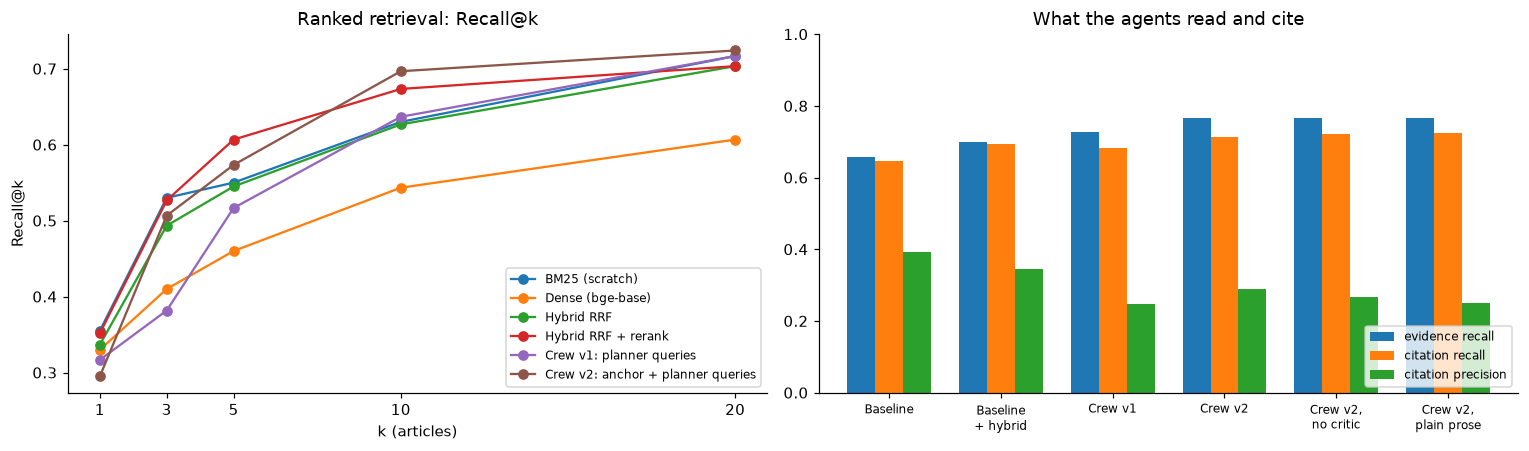
\includegraphics[width=0.85\textwidth]{retrieval.png}
\caption{Left: Recall@$k$ of the ranked retrievers. Right: evidence recall, citation recall and citation precision of
the agents.}
\label{fig:retrieval}
\end{figure*}

\subsection{Response accuracy}
Table~\ref{tab:main} and Fig.~\ref{fig:judge} give the main results. The judge metrics carry 95\% bootstrap confidence intervals in the
notebook; with 50 questions, fact-recall differences below about 0.06 are within noise.

\begin{table*}[t]
\caption{Response accuracy on CleanTech-50 (mean over 50 questions). FR = judge fact recall; Corr = judge
correctness (1--5); Faith = share of claims supported by the cited sources; Contr = contradicted key facts;
BERTS = rescaled BERTScore F1; cost and latency per question.}
\label{tab:main}
\centering
\begin{tabular}{lcccccccc}
\toprule
System & FR $\uparrow$ & Corr $\uparrow$ & Faith $\uparrow$ & Contr $\downarrow$ & BERTS $\uparrow$ & ROUGE-L $\uparrow$ & Cost (\$) & Latency (s) \\
\midrule
Closed-book (Sonnet 5.5)       & .474 & 3.06 & --   & .010 & .060 & .139 & .007 & 6.1 \\
Baseline (Part 1, ReAct)       & .672 & 3.76 & \textbf{.966} & .016 & .111 & \textbf{.176} & .022 & 6.9 \\
Baseline + hybrid retrieval    & .628 & 3.76 & .964 & .013 & \textbf{.112} & .172 & .022 & 9.4 \\
Crew v1                        & .559 & 3.40 & .927 & .029 & .070 & .160 & .173 & 55.8 \\
Crew v2                        & .603 & 3.62 & .926 & .040 & .080 & .164 & .175 & 43.5 \\
\quad v2, no critic (first draft) & .630 & 3.66 & .909 & .031 & .094 & .170 & -- & -- \\
\quad v2, plain prose (no STE) & \textbf{.683} & \textbf{3.84} & .915 & .024 & .097 & .165 & -- & -- \\
\bottomrule
\end{tabular}
\end{table*}

\begin{figure*}[t]
\centering
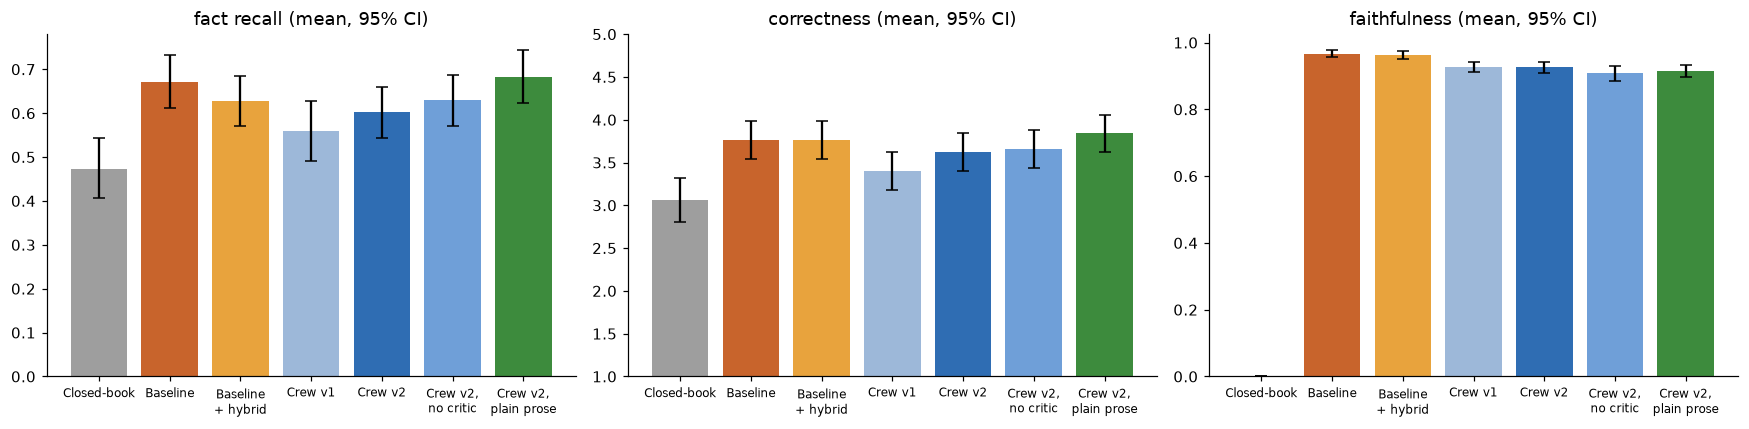
\includegraphics[width=0.92\textwidth]{judge_scores.png}
\caption{LLM-judge scores per system with 95\% bootstrap confidence intervals. Closed-book has no citations, so no faithfulness.}
\label{fig:judge}
\end{figure*}

\textbf{Retrieval is the largest effect.} Grounding the same model in the corpus raises fact recall from 0.474
to 0.672 and correctness from 3.06 to 3.76 (both $p<0.001$; 35 wins, 8 losses). The per-topic view
(Fig.~\ref{fig:topics}) shows why. Without retrieval, recall collapses on Geothermal (0.27), Policy (0.23) and
Solar (0.33), whose questions hinge on specific 2023 projects that no model saw in pre-training. It stays at 0.71 on
Climate \& Environment, where general science suffices.

\textbf{Answers are faithful.} 97\% of the baseline's claims and 93\% of the crew's are supported by the passages
they cite, and at most 4\% of key facts are contradicted. The output guardrail removed no hallucinated citation
in any answer: the writer cited only ids it had been shown.

\textbf{The multi-agent crew does not beat the single agent.} Crew v2 recalls fewer reference facts than the
baseline (0.603 vs 0.672, $p=0.002$) and is less faithful ($p<0.001$); the correctness gap is not significant
($p=0.07$). Its best configuration, the first draft re-written without the STE instruction, is the top system
on fact recall (0.683) and correctness (3.84), but it is only level with the baseline, at eight times the cost and
six times the latency.

\begin{figure}[t]
\centering
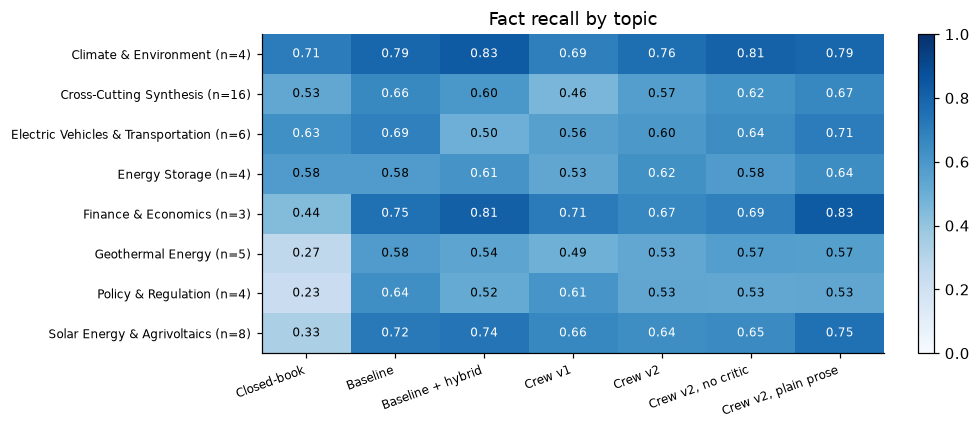
\includegraphics[width=\columnwidth]{topics.png}
\caption{Judge fact recall by topic and system (number of questions in parentheses).}
\label{fig:topics}
\end{figure}

\subsection{Ablations}
Because both ablations re-use v2's saved evidence, each changes exactly one component.

\textbf{ASD-STE100 trades content for readability.} The STE instruction works as intended
(Table~\ref{tab:ste}). The crew's sentences average 11 words against 23 in the references, 97\% fit the STE
limit, passive voice falls to 2\%, and Flesch Reading Ease rises from 16 (``very difficult'') to 50. On identical
evidence, however, the plain-prose writer recalls 5.2 points more key facts ($p<0.001$) and scores 0.18 higher on
correctness ($p=0.01$). Short sentences leave room for fewer facts in the same word budget, and STE's simplification
drops qualifiers that the reference counts as facts. This is a concrete, measured cost of Karpathy's suggestion:
STE answers are easier to \emph{review}, but on this task they are about 8\% less complete.

\begin{table}[t]
\caption{Readability and STE compliance (rule-based checker)}
\label{tab:ste}
\centering
\setlength{\tabcolsep}{4pt}
\begin{tabular}{lcccc}
\toprule
Text & Words/sent. & $\le$ limit & Passive & Flesch \\
\midrule
Reference answers      & 23.0 & 62\% & 10.0\% & 16 \\
Closed-book            & 16.8 & 83\% & 9.3\% & 31 \\
Baseline (Part 1)      & 12.1 & 99\% & 8.6\% & 43 \\
Crew v2 (STE)          & 11.0 & 97\% & 2.3\% & 50 \\
Crew v2, plain prose   & 16.8 & 84\% & 14.4\% & 37 \\
\bottomrule
\end{tabular}
\end{table}

\textbf{The critic adds cost, not measurable quality.} Comparing v2's final answer with its first draft, the critic
loop has no significant effect on fact recall ($-0.028$, $p=0.13$) or correctness ($p=0.56$). It nudges
faithfulness up ($+0.017$, $p=0.08$), which is its purpose. It requested a revision for 44 of 50 first drafts, and
most revisions added caveats rather than facts.

\textbf{Retrieval alone does not transfer to the baseline.} Giving the baseline the hybrid retriever raised its
evidence recall but left its answers unchanged (fact recall $-0.04$, $p=0.09$; correctness identical). A single
focused query per turn already finds what the agent needs for its answer; the extra articles mattered only in the
crew, where several researchers query different aspects.

\subsection{From v1 to v2: error analysis}
\label{sec:v2}
Crew v1 scored clearly below the baseline (fact recall 0.559). Inspecting its traces revealed three
implementation faults and two design faults:
(i) text read through \texttt{get\_article} or \texttt{summarize\_article} was cited but never recorded as
evidence;
(ii) the writer saw only the first 24 passages \emph{in arrival order}, so the last researcher's evidence could be
dropped;
(iii) the evaluation itself truncated cited sources to 9{,}000 characters, which penalised answers with many
citations (fixing it raised every system's measured faithfulness, the baseline's from 0.85 to 0.97);
(iv) decomposed queries lost the question's specificity (R@3 0.38); and (v) the critic demanded tangential
additions. v2 records all evidence, ranks passages by reranker score, adds the anchor query, and narrows the
critic. Fact recall rose to 0.603 ($p=0.08$) and correctness from 3.40 to 3.62 ($p=0.02$). Since these fixes were
motivated by errors on the test set itself, v2's scores are optimistic; v1 is the fair first-attempt result.

\subsection{Judge reliability and cost}
The judge's fact recall correlates with BERTScore at $\rho=0.54$ and with ROUGE-L at $\rho=0.48$: it tracks meaning,
but it is not simply a lexical metric. Re-grading 25 random answers with fresh calls gave the same correctness score
80\% of the time and never differed by more than one point (quadratic-weighted $\kappa=0.82$). All agent runs in this study
(Part~1, seven systems and both crew versions) cost \$24.67 in Anthropic API calls, as recorded by the usage
callbacks; the judge's OpenAI calls are billed separately.

\section{Discussion}
\textbf{Why does the crew not win?} The error analysis points to a mismatch between the system's search space and
the benchmark's construction. Every reference answer synthesizes 2--5 articles published in the same week, and
questions refer to them as ``the interviews and reports''. The crew searches 20{,}111 articles with several
researchers, so it finds the referenced articles more often than any other system. It then writes a broad,
well-supported survey from about seven sources, and the reference facts are crowded out. The three lowest-scoring
crew answers all follow this pattern. For Q21, the crew read the Diverso interview but answered ``barriers to
geothermal'' from thirteen permitting articles, and the judge rated it accurate yet off-target. The single ReAct
agent, by contrast, issues one or two focused queries and stays close to whatever it finds first, which on this
benchmark is usually the right article.

\textbf{What would help without overfitting?} A planner step that first resolves \emph{which} documents a question
refers to (by entity, outlet and date) and then restricts synthesis to them; a critic that runs only when the
draft contains unsupported claims; and STE applied as a presentation layer (a summary box) on top of complete
prose, instead of as a constraint on the answer itself.

\textbf{Limitations.} Fifty questions give wide confidence intervals; one judge model scores against one reference
per question, and its key facts come from the same judge; and article-level retrieval metrics penalise correct
answers drawn from other articles. Agent runs are stochastic (no temperature control on these models), so a
re-run would shift individual scores; the reported numbers come from one cached run.

\section{Conclusion}
I built an agentic RAG system for 20{,}111 cleantech articles with six extensions: a from-scratch BM25 with RRF and
reranking, an MCP tool server with a hand-written client, a planner/researcher/writer/critic crew with memory,
input and output guardrails, ASD-STE100 answers with a compliance checker, and scholarly search. A rigorous
evaluation shows that retrieval is the decisive component (+0.20 fact recall) and that BM25 beats dense
retrieval on this entity-heavy corpus. Multi-agent decomposition finds 17\% more of the referenced articles.
However, a single strong ReAct agent writes equally good answers at one eighth of the cost, and STE answers are far
more readable but less complete. More agents are not automatically better: each component has to earn its cost on
the target task, and only careful ablation shows which ones do.

\section{Reflection}
\emph{[Draft written from the project log; edit it so it is in your own words.]}
This project tied the whole course together. Cleaning the corpus was HW1 again: the duplicated ``blob''
paragraphs and tokenised apostrophes would have quietly corrupted every downstream number had I not looked at
raw rows first. The fact that BM25 beat a modern embedding model echoed HW2 and HW4: distributional vectors capture
similarity, but counting words still wins when the signal is a rare proper noun. HW3's RAG pipeline became
the Part~1 baseline, and HW5's lesson that ROUGE barely separates good summaries from mediocre ones is why the
LLM judge, not overlap metrics, is the primary measure here.

The most valuable moment was a negative result. My first multi-agent crew, the part I was most excited about,
scored clearly \emph{below} the simple baseline. Tracing its failures turned up two bugs in my own evaluation
code, which had penalised the crew, as well as real design flaws. Fixing them improved the crew, but the honest
conclusion is still that a single strong agent is hard to beat on this benchmark. I learned to budget as
much effort for measurement as for building, to run ablations that change exactly one thing, and to report cost
and latency next to accuracy, because an 8$\times$ more expensive system has to justify itself. Building the MCP
server and the parallel LangGraph crew also taught me practical engineering lessons that no tutorial covers: GPU
thread safety, async task ownership in Jupyter, and caching every expensive call so that results are reproducible.

Overall, the course moved from text processing and $n$-gram models to transformers, summarization and
retrieval-augmented agents, and each assignment supplied a tool or a lesson that this project needed. I leave it
far more skeptical of impressive-looking demos and more confident that I can evaluate NLP systems carefully.

\section*{Acknowledgment}
Claude (Anthropic) was used as a coding assistant. All design decisions, experiments and conclusions are my own and
were checked against the notebook outputs.


\bibliographystyle{IEEEtran}
\bibliography{refs}

\end{document}
